
\section{Experimental Evaluation}

\subsection{Experimental Setup}

 \begin{table*}
  \caption{Benchmarks Characteristics \cite{bienia08characterizationreport}\cite{woo1995splash}\cite{southern2016analysis}}
  \center
  \label{BC}
   \scalebox{1}{
   \begin{tabular}{ p{3cm} | p{3cm} | p{3cm} | p{3cm} | p{3cm} }
     \toprule[1pt]
     Name & Type of Parallelism & Synchronization Rate & Comm/Comp Ratio & Number Threads \footnote{$n$ is the input parameter.} \\
     \toprule[1pt]
    blackscholes & data-parallel & low & high & 1 + n \\
    bodytrack & data-parallel & medium & high & 2 + n\\
    dedup & pipline & medium & high & 3 + 3n\\
    ferret & pipline & high & medium & 3 + 4n\\
    fluidanimate & data-parallel & very high & low & 1 + n\\
   % freqmine & data-parallel & high & high &4\\
    swaptions & data-parallel & low & low & 1 + n\\
    radix & data-parallel & low & high & n\\
    lu\_ncb & data-parallel& low & low & n \\
    lu\_cb & data-parallel& low & low & n\\
    ocean\_cp & data-parallel & low & low & n\\
    water\_nsquared & data-parallel& medium & medium & n\\
    water\_spatial & data-parallel& low & low & n\\
    fmm & data-parallel& medium & low & n\\
    fft & data-parallel& low & high & n\\
      \midrule
     \bottomrule
  \end{tabular}}
\end{table*}

 \begin{table*}
  \caption{Benchmarks Compositions New}
  \center
  \label{BCN}
   \scalebox{1}{
   \begin{tabular}{ p{2cm} | p{7cm} | p{4cm} | p{2cm} }
     \toprule[1pt]
     \multicolumn{4}{c}{Synchronization-intensive VS Non-synchronization-intensive Workloads}\\
     \midrule
     Index & Workload Composition & Synchronizations & Threads \\
     \toprule[1pt]
    Sync - 1 & water\_nsquared - fmm & intensive & 4 \\
    Sync - 2 & dedup - fluidanimate & intensive & 18 \\
    Sync - 3 & water\_nsquared - fmm - fluidanimate - bodytrack & intensive & 9 \\
    Sync - 4 & dedup - ferret - fmm - water\_nsquared & intensive & 20\\
      \midrule
    NSync - 1 & radix - fft & non-intensive & 4 \\
    NSync - 2 & blackscholes - swaptions & non-intensive & 16 \\
    NSync - 3 & radix - fft - water\_spatial - lu\_cb & non-intensive & 8\\
    NSync - 4 & blackscholes - ocean\_cp - lu\_cb - swaptions & non-intensive & 20\\
   %  \bottomrule
      \toprule[1pt]
     \multicolumn{4}{c}{Communication-intensive VS Computation-intensive Workloads}\\
     \midrule
     Index & Workload Composition & Comm/Comp & Threads \\
     \toprule[1pt]
    Comm - 1 & water\_nsquared - fft & Communication-intensive & 4 \\
    Comm - 2 & radix - blackscholes &  Communication-intensive & 16 \\
    Comm - 3 & water\_nsquared - fft - radix - blackscholes &  Communication-intensive & 8 \\
    Comm - 4 & bodytrack - dedup - ferret - fft &  Communication-intensive & 20\\
      \midrule
    Comp - 1 & water\_spatial - fmm & Computation-intensive & 4 \\
    Comp - 2 & fluidanimate - swaptions & Computation-intensive & 16 \\
    Comp - 3 & lu\_ncb - fmm - water\_spatial - lu\_cb & Computation-intensive & 8\\
    Comp - 4 & fluidanimate - ocean\_cp - lu\_cb - swaptions & Computation-intensive & 20\\
     \bottomrule
     
  \end{tabular}}
\end{table*}

 \begin{table*}
  \caption{Workloads Compositions}
  \center
  \label{WC}
   \scalebox{0.9}{
   \begin{tabular}{p{1.5cm} |p{5.5cm} || p{1.5cm} |p{9cm} }
     \toprule[1pt]
     \multicolumn{4}{c}{Random-mixed Workloads from PARSEC3.0 and SPLASH-2}\\
     \toprule[1pt] 
    2B-1 &blackshcoles - radix &4B-1 &blackshcoles - bodytrack - radix - lu\_ncb\\
    2B-2 &fft - swaptions &4B-2 &water\_spatial - fmm - fft - fluidanimate\\
    2B-3 &lu\_cb - dedup  &4B-3 &lu\_cb - water\_nsquared - fmm - freqmine\\
    2B-4 &lu\_ncb - bodytrack &4B-4 &lu\_cb - lu\_ncb - bodytrack - dedup\\
    2B-5 &ferret - fluidanimate &4B-5 &radix - lu\_ncb - lu\_cb - fft\\
    2B-6 &freqmine - water\_nsquared &4B-6 &blackscholes - bodytrack - dedup - fluidanimate\\
    2B-7 &ocean\_cp - fft &4B-7 &radix - ocean\_cp - blackscholes - swaptions\\
    2B-8 &ferret - water\_spatial &4B-8 &water\_spatial - water\_nsquared - ferret - freqmine\\
    2B-9 &fluidanmiate - fmm &4B-9 &fmm - water\_spatial - ferret - swaptions\\
    2B-10 &fmm - water\_spatial &4B-10 &ocean\_cp - fft - fluidanimate - swaptions\\
  %  6B-M &blackshcoles,bodytrack,dedup,radix,lu\_ncb,lu\_cb\\
  %  8B-M &blackshcoles,bodytrack,dedup,fluidanmiate,radix,lu\_ncb,lu\_cb,radiosity\\
  %  12B-M &blackshcoles,bodytrack,dedup,fluidanmiate,streamcluster,swaptions,radix,lu\_ncb,lu\_cb,radiosity,ocean\_cp,fft\\    
     \midrule
 %    \toprule[1pt]
 %    \multicolumn{4}{c}{Multi/Single-thread multiprogrammed Workloads from PARSEC3.0, SPLASH-2 and SPEC2006}\\
 %    \toprule[1pt]  
 %   3B-1 &blackshcoles - radix - mcf &6B-1 &blackshcoles - bodytrack - radix - lu\_ncb - mcf - bzip2\\
  %  3B-2 &fft - swaptions - mcf &6B-2 &fft - radix - blackscholes - fluidanimate - mcf - bzip2\\
   % 3B-3 &freqmine - swaptions - mcf &6B-3 &blackscholes - dedup - freqmine - swaptions - mcf - bzip2\\
%    3B-4 &blackscholes - freqmine - bzip2 &6B-4 &lu\_cb - lu\_ncb - bodytrack - dedup - mcf - bzip2\\
    %3B-5 &ocean\_cp - fluidanimate - mcf &6B-5 &radix - lu\_ncb - lu\_cb - fft - mcf - bzip2\\
 %   3B-5 &radix - lu\_ncb - bzip2 &6B-5 &radix - lu\_ncb - lu\_cb - fft - mcf - bzip2\\
  %  3B-6 &fluidanimate - freqmine - bzip2 &6B-6 &blackscholes - freqmine - swaptions - fluidanimate - mcf - bzip2\\
   % 3B-7 &blackscholes - fluidanimate - bzip2 &6B-7 &lu\_ncb - ocean\_cp - bodytrack - swaptions - mcf - bzip2\\
%    3B-8 &dedup - fluidanimate - bzip2 &6B-8 &lu\_cb - ocean\_cp - dedup - swaptions - mcf - bzip2\\
 %   3B-9 &lu\_cb - swaptions - bzip2 &6B-9 &ocean\_cp - fft - fluidanimate - swaptions - mcf - bzip2\\
 %   7B-MS   &blackshcoles,bodytrack,dedup,radix,lu\_ncb,lu\_cb,mcf\\
 %   11B-MS &blackshcoles,bodytrack,dedup,canneal,swaptions,radix,lu\_ncb,lu\_cb,radiosity, bzip2,mcf\\ 
  %  15B-MS &blackshcoles,bodytrack,dedup,fluidanmiate,streamcluster,canneal,swaptions,radix,lu\_ncb,lu\_cb,radiosity, ocean\_cp,fft,bzip2,mcf\\   
  % &6B-7 &radix - ocean\_cp - blackscholes - swaptions - mcf - bzip2\\
    \bottomrule
  \end{tabular}}
\end{table*}

\textbf{\textit{Experimental Environment:}} We ran our experiments on GEM5, simulating an ARM big.LITTLE-like architecture. The big cores are similar to out-of-order 2 GHz CortexA57 cores, with a 49 KB L1 instruction cache, a 32 KB L1 data cache, and a 2 MB L2 cache. The little cores are similar to in-order 1.2 GHz CortexA53 ones, with a 32 KB L1 instruction cache, a 32 KB L1 data cache, and a 0.5 MB L2 cache. We evaluated two distinct hardware configurations, one with two big and two little cores and one with four big and four little ones. The OS is Linux v3.16. We cross-compiled the kernel with gcc v5.4.0, while we compiled the benchmarks inside the emulated environment with gcc v4.8.2.

\textbf{\textit{Workloads:}} For our workloads we used 17 different benchmarks. Fifteen are multi-threaded pulled either from PARSEC3.0~\cite{bienia11benchmarking} ({\it blackscholes, bodytrack, dedup, swaptions, freqmine, ferret and fluidanmiate}) or from SPLASH2~\cite{woo1995splash} ({\it radix, lu\_ncb, lu\_cb, ocean\_cp, water\_nsquared, water\_spatial, fmm and fft}). We added another two single-threaded benchmarks ({\it mcf, bzip2}) from SPEC CPU2006~\cite{henning2006spec} to complicate scheduling decisions. All benchmarks use pthread-based parallelism apart from \emph{freqmine} which does not support pthreads, only OpenMP. To keep the simulation time reasonably short, we use the \emph{simsmall} inputs for the multi-threaded benchmarks.

For \emph{mcf} we use the reference input, while for \textit{bzip2} we used the source reference input. We edited the source files of \textit{mcf} and \textit{bzip2} to limit the number of iterations of their outermost loops to 3000 for the former and 250 for the latter, to keep their runtimes in the same order of magnitude as the multi-threaded benchmarks.

%It is a common issue that GEM5 simulator does not support all PARSEC3.0 benchmarks well \cite{endo2014micro}, so we also applied several more SPLASH2 benchmarks \cite{woo1995splash}: {\it radix, lu\_ncb, lu\_cb, ocean\_cp and fft}. We also considered two more single-thread benchmarks ({\it mcf, bzip2}) from SPEC2006 \cite{henning2006spec} to make the tested multiprogrammed workloads further complicated. 
We randomly mix our selected benchmarks to build workloads with either multiple multi-threaded applications or mixed multiple multi-threaded and single-thread applications. Table~\ref{WC} shows the workloads we used. For all workloads, we boot the simulated system, start the benchmarks, and wait until they reach the end of their initialization. This is done with fast simulation. When all benchmarks are initialized, we switch to cycle accurate simulation and resume the execution of the benchmarks. We only collect statistics for the cycle accurate part of the simulation.

Each one of our results represents the average over two simulations with different core orders - either big cores first or little cores first. The initial state of the system can have a significant impact on performance. For the Linux scheduler in particular, the order of starting benchmarks will decide which benchmarks will be initially assigned to big and little cores. By randomizing the initial state and especially the execution order of the workload benchmarks for each simulation, we minimize the effect of randomness on our evaluation.

%The number of parallel threads for benchmarks from SPLASH2 can be setup easily as in input arguments, while for PARSEC benchmarks, we only setup the lower bound of threads and the program will then determines the actual number of threads based on the relationships described in \cite{southern2016analysis}. To avoid dominating system performance by a single benchmark in each workload, we normalized the number of threads from different benchmarks to be similar and keep the input sizes of all applications to be {\it simsmall}. 
%The only exception is on benchmark {\it streamcluster} from PARSEC3.0 - it is a known issue \cite{southern2016analysis,roth2012deconstructing} that increasing the number of threads to be greater than 4 will significantly decrease the performance of this benchmark because of its barrier based synchronization.

\textbf{\textit{Metrics:}} Our evaluation uses two metrics to quantify scheduling efficiency: {\it Heterogeneous Average Normalized Turnaround Time} (H\_ANTT) and {\it Heterogeneous System Throughput} (H\_STP). They are based on ANTT and STP, as introduced in~\cite{eyerman2008system}. For an application mix, both ANTT and STP use the runtime of each application when executed on its own, i.e. when there is no resource sharing and scheduling decisions have little effect. ANTT expresses the average slowdown of all applications in the mix, with the slowdown for each application being relative to its isolated runtime. STP expresses the sum of the relative throughputs for all applications, again relative to the isolated throughput.

For AMPs, these two metrics fail to work as intended. The runtime when executed alone is still affected by scheduling decisions, e.g. which threads to run on big cores. To overcome the problem, our modified metrics H\_ANTT and H\_STP use the runtime of each application in the mix when executed alone \emph{on a system where there are only big cores}. If the turnaround time of each application $i$ while being co-scheduled is $T^{M}_i$ and the turnaround time for the same application when running alone on a big-only system is $T^{SB}_i$, then:

$$ H\_ANTT = \frac{1}{n}\sum^{n}_{i=1}\frac{T^{M}_i}{T^{SB}_i}$$
$$ H\_STP = \sum^{n}_{i=1}\frac{T^{SB}_i}{T^{M}_i}$$

When we evaluate a single benchmark on its own, we use the {\it Heterogeneous Normalized Turnaround Time} (H\_NTT):

$$ H\_NTT = \frac{T^{M}}{T^{SB}}$$

H\_ANTT and H\_NTT are better when lower, H\_STP is better when higher. For most figures, we further normalize our results relative to the Linux CFS results for the same configuration and workload.

\textbf{\textit{Schedulers:}}
We compare COLAB against the Linux CFS scheduler~\cite{molnar2007cfs} and a scheduler based on WASH~\cite{jibaja2016portable}. WASH is implemented inside a Java VM and is meant to control the affinities of Java threads only. Our implementation uses the same heuristic as the original WASH but is part of the Linux scheduler and controls all application threads. Additionally, we replaced the WASH core sensitivity model with one built from scratch for our hardware configuration and our set of performance counters, using the same process as described in the WASH paper.

\begin{figure}
\centering
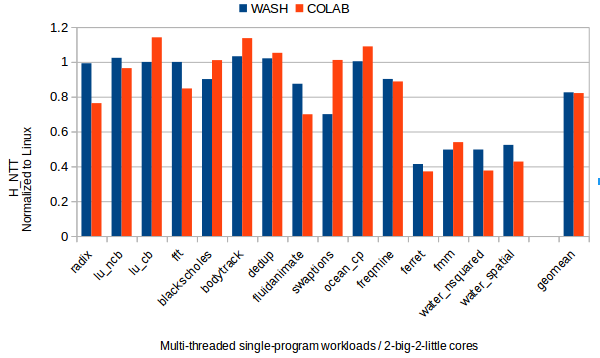
\includegraphics[scale=0.42]{figures/MSW4.png}
\caption{Heterogeneous Normalized Turnaround Time (H\_NTT) of single program workloads.  All results are normalized to the Linux CFS ones. Lower is better}
\label{MSW}
\end{figure}  
\begin{figure*}
\centering
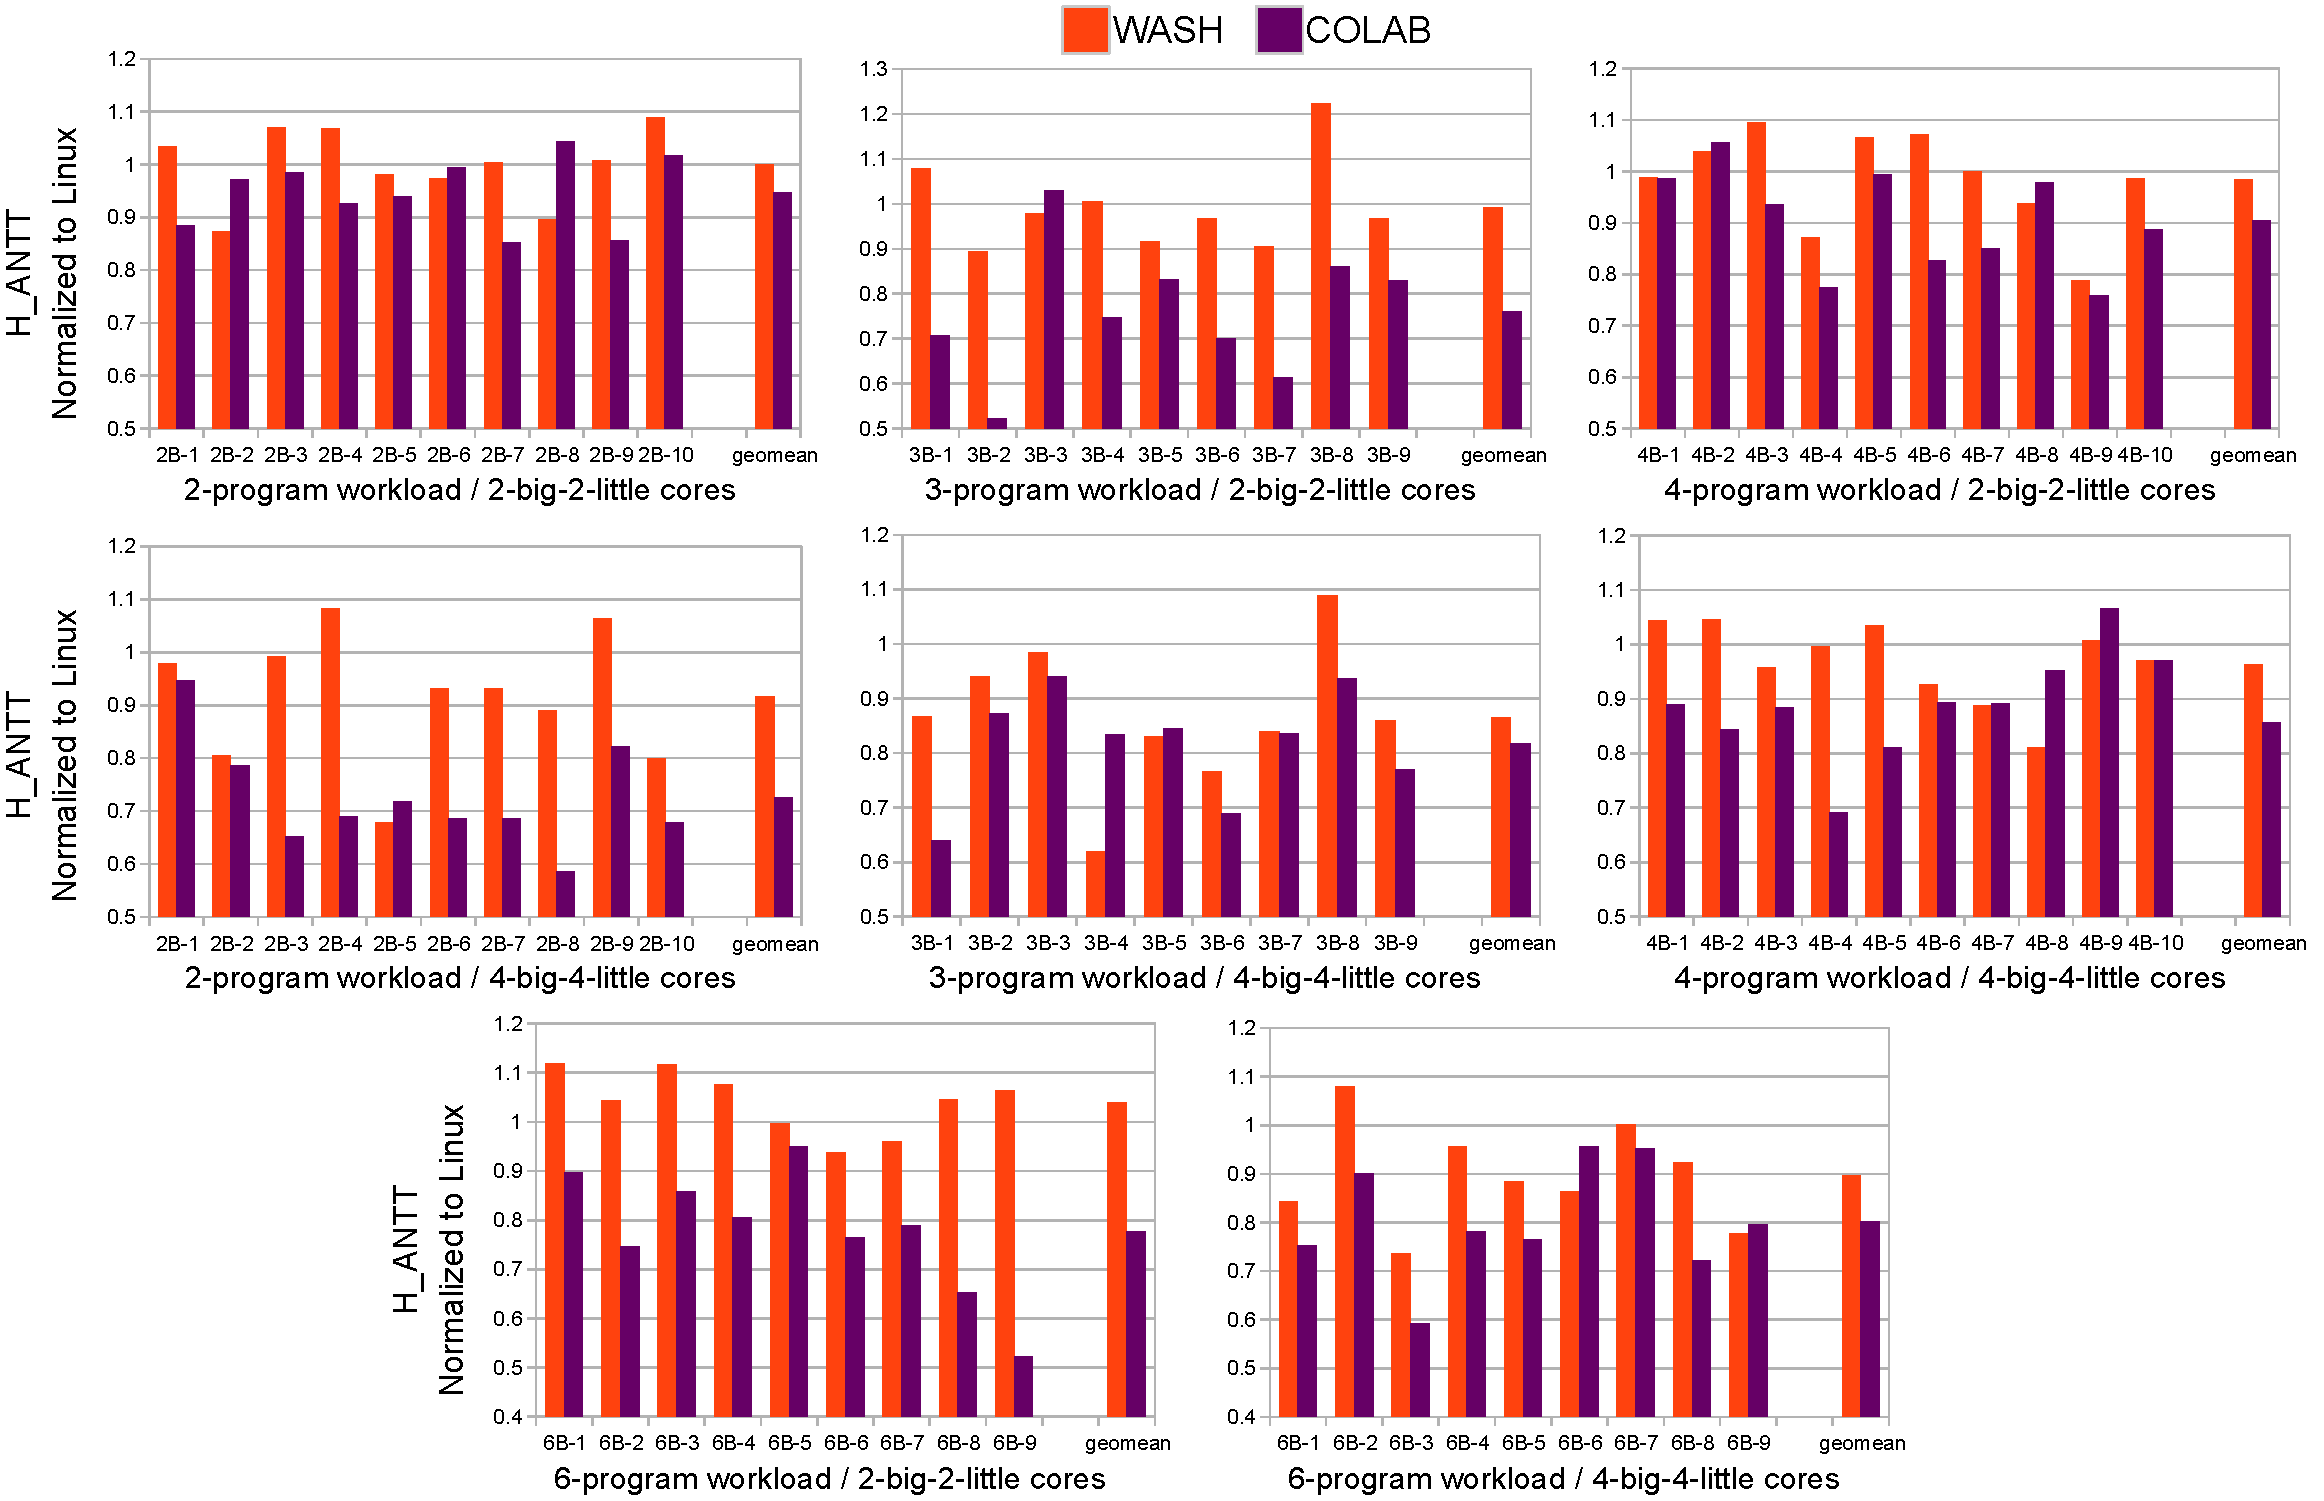
\includegraphics[scale=0.4]{figures/HANTT_NEW.pdf}
\caption{Heterogeneous Average Normalized Turnaround Time (H\_ANTT) of multiprogrammed workloads on 2-big-2-little and 4-big-4-little configurations. All results are normalized to the Linux CFS ones. Lower is better.}
\label{M24W}
\end{figure*}


\subsection{Experimental Results and Analysis}

\subsubsection{Single-programmed Workloads}
Much of the research on AMP scheduling focuses on single-programmed workloads. In this context, fairness and load balancing are not important, the focus is on core sensitivity and bottleneck acceleration. In this section, we examine how COLAB fares under this scenario. Figure~\ref{MSW} shows Heterogeneous Normalized Turnaround Time for all our multi-threaded benchmarks when executed alone on a 2-big-2-little hardware configuration. For each configuration and benchmark we present two bars, WASH (blue), COLAB(red). We do not present results for our two single-threaded benchmarks: scheduling them optimally for performance is trivial.

The AMP-agnostic Linux scheduler is inappropriate for most benchmarks. COLAB improves H\_NTT by up to 58\% and by 12\% on average. Our best result relative to Linux is for \emph{ferret}. Most computation happens in a pipeline pattern but its stages are not balanced. AMP-aware schedulers take advantage of that by scheduling the longest stages, the bottleneck threads, on big cores. As a result, COLAB does only 13\% worse than running on a system \emph{with four big cores}, while CFS executes the benchmark 173\% slower.

Our best result relative to WASH is for \emph{fluidanimate}. Previous work~\cite{bienia08characterization} has shown that \emph{fluidanimate} has around 100x more lock-based synchronizations than other PARSEC benchmarks. Our collaborative core allocation and thread selection policy is much better than WASH at prioritizing bottleneck threads.  As a result, we reduce turnaround time by 30\% compared to Linux and 20\% compared to WASH.

In some cases, such as \emph{bodytrack}, \emph{dedup}, \emph{lu\_ncb}, or \emph{freqmine}, AMP-awareness has little effect on performance. Such benchmarks split work dynamically between threads, so they adapt to asymmetries in processing speed. Moreover, all threads executed the same code and display similar core sensitivity, so there is no benefit in assigning specific threads to specific cores. When either WASH or COLAB interfere with scheduling decisions, they are more likely to make wrong decisions or introduce overhead than help. Such behavior was also apparent in the original WASH paper~\cite{jibaja2016portable}.

There is only one case where COLAB performs significantly worse than WASH. For \emph{swaptions}, we perform as well as the AMP-agnostic Linux scheduler while WASH improves turnaround time by 31\%. This is because the bottleneck threads of \emph{swaptions} are core insensitive while the non-bottleneck threads are core sensitive. This being the ideal case for WASH, it improves turnaround time while we fail to do the same.

On average, WASH and COLAB perform similarly well and improve performance by 12\% compared to Linux when handling single program workloads. This is a limited scenario, with no need for fairness and a simple decision space. COLAB was not expected to perform much better than the state-of-the-art, doing as well as it is a positive result.

\subsubsection{Multi-programmed Workloads}
Multi-threaded multi-program scheduling is the general scheduling case and the one where COLAB can have the largest impact. We examined its performance under two different hardware configurations (2-big-2-little and 4-big-4-little) and the 38 different workloads listed in Table~\ref{WC}, each workload comprised of two, three, four, or six programs.

\textbf{\textit{Heterogeneous Average Normalized Turnaround Time:}}
Figure~\ref{M24W} shows the Heterogeneous Average Normalized Turnaround Time (H\_ANTT) for all evaluated combinations of hardware and workload. The hardware configuration is indicated on the X-axis of each subplot. Lower H\_ANTT translates into higher performance.

With co-executed programs interfering with the communication patterns of each other, accelerating bottlenecks and critical threads becomes much more important. As a result, COLAB improves turnaround time by up to 48\% compared to Linux and up to 51\% compared to WASH. On average, COLAB outperforms the Linux scheduler by 5.3\% to 27.5\%  depending on the configuration, while it outperforms WASH by 5.2\% to 25.3\% for different numbers of cores and co-scheduled programs. As a general rule, the benefits of using COLAB over the default Linux scheduler become more pronounced with more cores, while it is the opposite case when compared to WASH.

The state-of-the-art WASH scheduler shows its limitations when used on a limited 2-big-2-little configuration. With increasing pressure from co-executed applications, especially single-threaded ones, properly balancing bottleneck acceleration and core sensitivity across multiple programs using only two big cores becomes difficult. For instance,  both \emph{dedup} and \emph{fluidanimate} are limited by frequent synchronizations. WASH identifies these bottlenecks and assigns their threads to big cores without further consideration. Instead of accelerating the bottleneck threads, this leads to the bottleneck threads getting stuck waiting for CPU time in busy runqueues. At the same time, non-critical threads enjoy short waiting times on little cores. For workloads that include these two benchmarks (2B-9, 3B-8, 4B-3), WASH ends up performing up to 20\% worse than Linux CFS. COLAB handles bottleneck threads in a more holistic way, improving performance by 7\% to 14\% for the same workloads.

Such issues become more pronounced the higher the pressure on the scheduler. When handling more benchmarks than the number of cores WASH tends to be worse than Linux. In the case of 6-program workloads on the 2-big-2-little system, WASH does worse for seven out of nine workloads. Our approach faces no problems, always doing better than Linux and producing a 23\% performance gain on average. As a matter of fact, COLAB thrives under such scenarios: more pressure on the scheduler means more interference between programs, more asymmetry and bottlenecks, and more potential for acceleration.

With more high performance cores, waiting times in big core runqueues fall and WASH behaves better. For 4-big-4-little systems, WASH achieves on average a 9\% performance gain against Linux. Still, our approach uses the processing resources more efficiently. It is better than WASH for 26 out of the 38 workloads, improving H\_ANTT by 11\% on average.

Co-scheduling single-threaded programs with multi-threaded ones tends to lead to suboptimal decisions for CFS and WASH. Single-threaded programs do not generally block, unless for I/O, so they might spend a long time running and forcing other thread in their runqueue to wait. CFS will occasionally place single-threaded programs in big cores, while WASH will do the same when the program is core sensitive. This means that bottleneck threads might end up spending a considerable amount of time waiting on big core runqueues for single-threaded programs to use their CPU time. COLAB, instead, will prioritize scheduling bottleneck threads, as long as it does not affect fairness. For workloads containing single-threaded benchmarks, our approach outperforms WASH for 30 out of 36 cases and CFS for 35 out of 36 cases. 

Overall, COLAB reduces the average turnaround time compared to CFS for 72 out of 76 cases. Even for the four cases where we do worse, the slowdown is less than 5\% and is due to the same effect discussed in the previous subsection: 
benchmarks with parallel patterns that can accommodate asymmetry without scheduler help combined with the overhead of a more proactive scheduler. Compared to WASH, we improve performance for 64 out of 76 cases.

\begin{figure*}
\centering
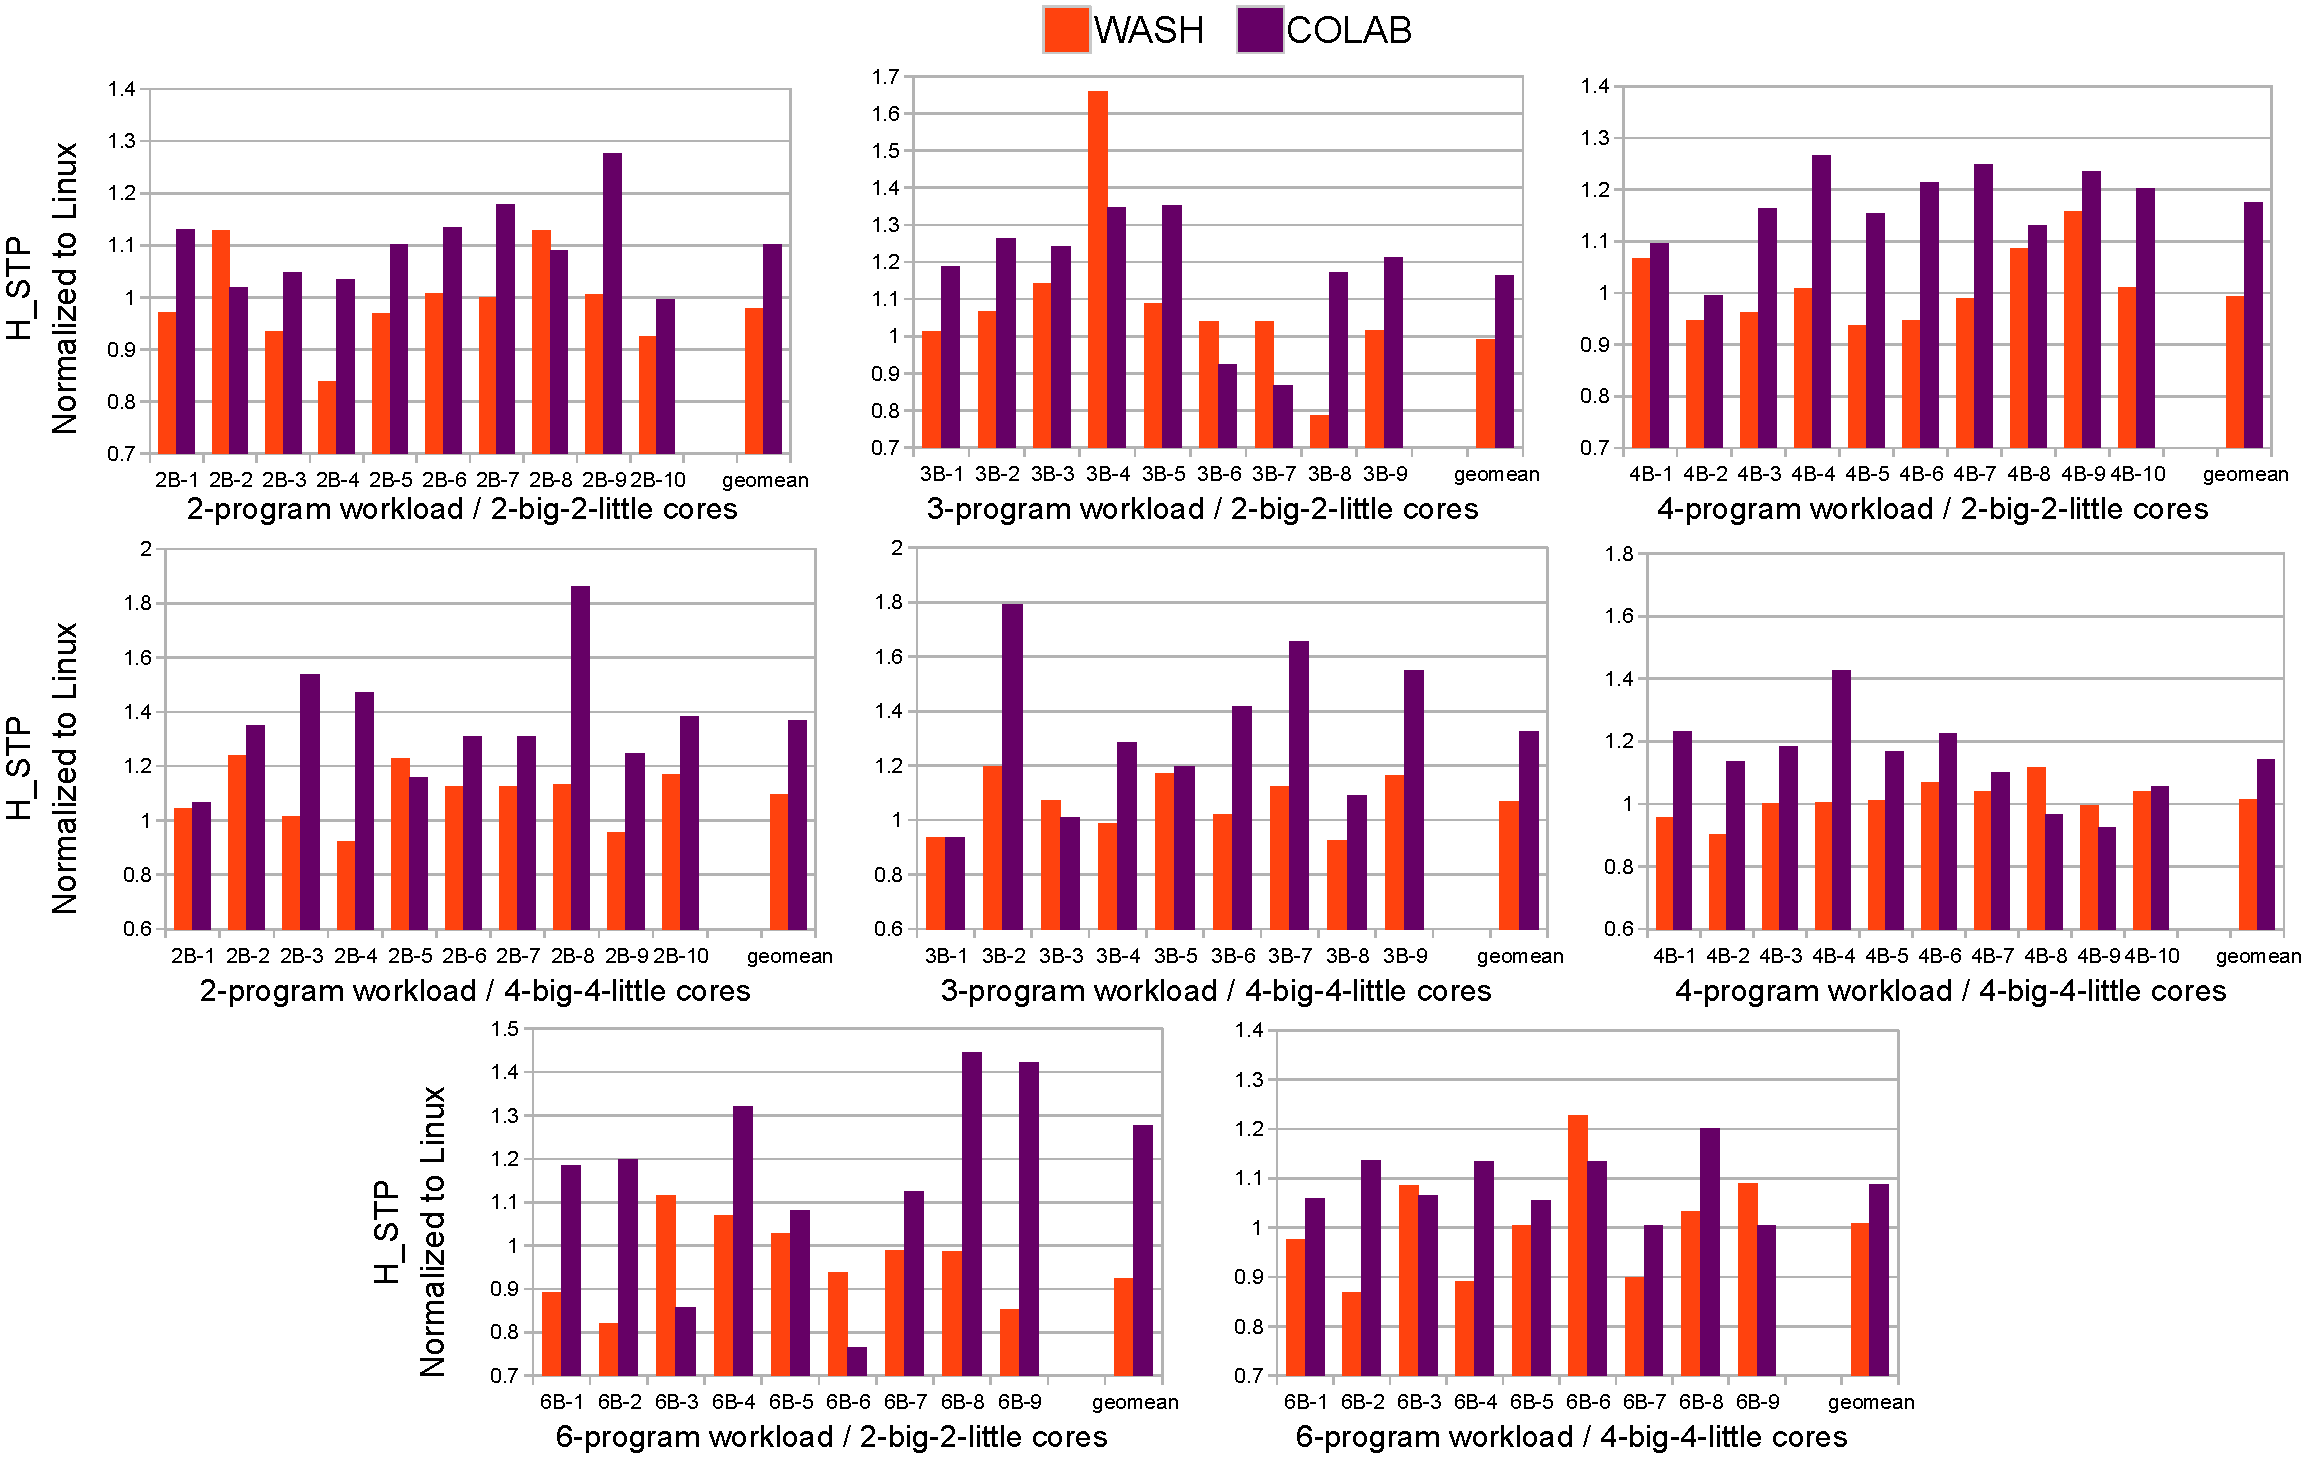
\includegraphics[scale=0.4]{figures/HSTP_NEW.pdf}
\caption{Heterogeneous System Throughput (H\_STP) of multiprogrammed workloads on 2-big-2-little and 4-big-4-little configurations. All results are normalized to the Linux CFS ones. Higher is better.}
\label{M36W}
\end{figure*} 
\textbf{\textit{Heterogeneous System Throughput:}}
Figure~\ref{M36W} shows our results for Heterogeneous System Throughput (H\_STP). As in the previous subsection, each subplot contains data for one hardware configuration and a specific number of co-scheduled programs.

Linux CFS and WASH do slightly better than COLAB in a few cases as our policy targets turnaround time optimization and will make decisions that hurt throughput in order to maintain some fairness. Still, on average our approach does better than CFS and WASH for most configurations. For certain asymmetric multi-program workloads, COLAB achieves not only acceptable throughput but significant improvement over its competition. By distributing bottleneck threads more evenly across cores, it makes better use of the system resources, avoiding leaving cores idle. This translates into up to 86\% higher throughput performance gain on the 4-big-4-little system, for 2B-8, and up-to 44\% higher throughput on the 2-big-2-little system, for 6B-8.
%Towards all 76 individual cases, other approaches only better than us on 3 cases and our approach only less than 10\% worse than them in the worst case (3B-6 on the 2-big-2-little configuration). 
%The collaboration-only approach can also do better than both Linux and WASH in most cases but worse than our final approach equipped with the multi-factor Coordinated model.

%with up-to 34\% improvement of H\_STP against other approaches. It does at most 15\% worse than WASH in the worst case (2B-2). Linux can also do slightly better than both WASH and our approach for some workloads (2B-10). As for the geomean of the multiple tests, our approach results in around 5\% performance gain of H\_ANTT against Linux CFS, while both WASH and the collaboration-only approach can not do better than Linux. The collaboration-only approach can achieve around 5\% improvement of H\_STP against Linux and WASH, and the improvement grows up to more than 10\% by applying our final approach. 

%The results on 4-benchmark workloads are shown in the lower two graphs of figure \ref{M24W}.Our approach can achieve up-to 39\% performance gain of H\_ANTT on certain workloads (4B-7) and up-to 40\% improvement of H\_STP on (4B-7). It does at most 10\% worse than WASH in the worst case (4B-9). Linux can also do better than both WASH and our approach for some workloads (4B-9). As for the geomean of the multiple tests, both the collaboration-only and our final approach results in around 9\% performance gain of H\_ANTT against WASH and 7\% against Linux. The collaboration-only approach can achieve around 14\% improvement of H\_STP against Linux and WASH, and the improvement grows up to more than 19\% by applying our final approach.  

%\textbf{\textit{Multi/single-thread Multi-program Workloads}}
 
%The results on 3-benchmark workloads are shown in the upper two graphs of figure \ref{M36W}.
%Our approach can achieve up-to 54\% performance gain of H\_ANTT on certain workloads (3B-2) and up-to 33\% improvement of H\_STP on (3B-1). It can always keep better than WASH in the all workload cases. Linux can also do slightly better than both WASH and our approach for some workloads (3B-6). As for the geomean of the multiple tests, the collaboration-only approach obtains around 5\% performance gain of H\_ANTT against Linux and WASH is not better than Linux. Our final approach can achieve 20\% performance gain against Linux and 25\% against WASH. The collaboration-only approach can achieve around 13\% improvement of H\_STP against Linux and WASH, and the improvement grows up to more than 18\% by applying our final approach.  
 
%The results on 6-benchmark workloads are shown in the lower two graphs of figure \ref{M36W}.
%Our approach can achieve up-to 54\% performance gain of H\_ANTT on certain workloads (6B-3) and up-to 46\% improvement of H\_STP on (6B-4). Linux can also do slightly better than both WASH and our approach for some workloads (6B-1,6B-5). As for the geomean of the multiple tests, the collaboration-only approach obtains around 17\% performance gain of H\_ANTT against Linux and WASH is not better than Linux. Our final approach can achieve 23\% performance gain against Linux and 27\% against WASH. The collaboration-only approach can achieve around 16\% improvement of H\_STP against Linux and WASH, and the improvement grows up to more than 20\% by applying our final approach.  



\textbf{\textit{Experimental Summary}} As shown in the results, the state-of-the-art AMP-aware WASH scheduler struggles to make good decisions as the number of co-scheduled programs rises. Trying to handle both core sensitivity and bottleneck acceleration through thread affinity alone may lead to too many threads assigned to big cores. Instead, we handle the two optimization aims separately. We assign on big cores only threads which run significantly faster on them and we prioritize running bottleneck threads regardless of their thread affinity. This leads to improved turnaround time, higher throughput, and better use of the processor resources compared to both CFS and WASH.